% s6results.tex

\ac{S6} began on 7 July 2009 and ran until 20 October 2010. It overlapped two Virgo runs: \ac{VSR2}, which ran from 7 July 2009 to 11 January 2010, and \ac{VSR3}, which ran from 11 August 2010 to 20 October 2010. A number of improvements were made in both instrument hardware and \ac{CBC} analysis software between \ac{S5} and \ac{S6}. The software improvements have already been detailed in prior chapters: New \ac{SNR} was developed to replace effective \ac{SNR}, and Pipedown was implemented.

In this chapter we detail the \ac{S6} and VSR2/3 analysis. Section \ref{sec:hardware_improvements} describes some of the hardware improvements made to the detectors between \ac{S5} and \ac{S6}. In section \ref{sec:s6_epochs} we describe each of the four epochs the analysis was broken into. Section \ref{sec:dq_issues} details some of the major \ac{DQ} issues that arised during \ac{S6} and how they were dealt with, along with tuning decisions made. In this section we give an example of a veto developed from the loudest-slide studies that were implemented in the second half of \ac{S6}. Finally, in section \ref{sec:s6_results_and_big_dog} we give the results of the search, and we describe a blind injection that was made, and found, during \ac{S6}/VSR3. We do not present upper limits here as they are still being computed.

\section{Hardware Improvements}
\label{sec:hardware_improvements}

The two $4\,$km \ac{LIGO} interferometers, H1 and L1, were used for \ac{S6}.
The $2\,$km Hanford detector, H2, that is described in the last chapter was not
operational. Several hardware changes were made to the \ac{LIGO} detectors so
that prototypes of advanced LIGO technology could be installed and tested. This
included the installation of a more powerful, $35~\mathrm{W}$ laser, and the
implementation of a DC readout system that included a new Output Mode Cleaner
on an advanced LIGO seismic isolation table~\cite{Adhikari:2006}. In addition,
the hydraulic seismic isolation system was improved by fine-tuning its
feed-forward path. Known as HEPI feed-forward, this improvement was implemented
in January of 2010; it is described in more detail in section \ref{sec:s6b},
below.

Several hardware enhancements were also made to the Virgo detector in the
period between \ac{VSR1} and \ac{VSR2}. A more powerful laser was installed,
along with a thermal compensation system and scattered light was better
mitigated. During early 2010, monolithic suspension was installed, which
involved replacing Virgo's test masses with new mirrors hung from fused-silica
fibers. Following this upgrade Virgo began \ac{VSR3}. 

The average sensitivity of the detectors to binary coalescence signals in each epoch is shown
in Figures \ref{fig:s6a_insprange} -- \ref{fig:s6d_insprange}. These figures show the distance at
which an optimally oriented and located binary would produce a \ac{SNR}
of $8$ in a given detector. The figures show how the detectors were improved over the course of the run, until the eventually surpassed the best \ac{S5} ranges. 
%The reduction in the horizon distance of the Virgo detector in \ac{VSR3} is
%due to a mirror with an incorrect radius of curvature being installed
%during the conversion to monolithic suspension.

\section{S6 Epochs}

\ac{S6} and VSR2/3 were broken into four epochs: \emph{S6A}, which ran from 7 July 2009 to 1 September 2009; \emph{S6B}, 24 September 2009 to 11 January 2010; \emph{S6C}, 6 February 2010 to 25 June 2010; \emph{S6D}, 26 June 2010 to 20 October 2010. Figure \ref{fig:s6_insprange_v_time} shows a plot of the \ac{BNS} inspiral range (with each component mass $= 1.4\,\Msun$) across all of \ac{S6} and the span of each epochs. The start and end times of the epochs were based on a combination of instrumental and analysis factors. S6A ended at a pre-planned commissioning break to try to improve the detectors after learning lessons from the first two months of running. S6B ran from the end of the commissioning break until the end of \ac{VSR2}. At this point, Virgo was taken off line for eight months in order to install the monolithic suspension. S6C therefore consisted only of double coincident time between Hanford and Livingston. Another commissioning break was taken at the end of S6B, hence the gap between the end of S6B and the start of S6C. S6D was to begin when Virgo came back online in August of 2010. However, during S6C we noticed that templates with total masses $> 25\,\Msun$ often rang off due to glitches. Thus we decided to lower the low-mass template bank from $2 \leq \mtotal/\Msun \leq 35$ to $2 \leq \mtotal/\Msun \leq 25$. We wanted to do this as soon as possible, and so the somewhat arbitrary date of 26 June 2010 was chosen as the break between S6C and S6D. Aside from Virgo eventually coming back online, there were no major instrumental adjustments between S6C and D. There were, however, new vetoes implemented for S6D based on \ac{CBC} results in S6C. These new vetoes, as well as more details about the decision to lower the template bank, are discussed in section \ref{sec:dq_issues}. In the next few sections we give more details about each of the epochs.

\subsection{S6A}

Being the start of a new Science run, the \ac{LIGO} detectors had lower sensitivity and more glitches in S6A than in later epochs. This can be seen in Figure \ref{fig:s6_insprange_v_time}. In fact, the S6A \ac{LIGO} ranges were somewhat lower than they had been during their peak sensitivity in \ac{S5}. Figure \ref{fig:s6a_insprange} shows the average inspiral range versus binary total mass during S6A as compared to best ranges of \ac{S5}. We can see that Virgo, however, showed much improvement over VSR1, and had better sensitivity than H2 at its best in \ac{S5}.

In the \ac{S5}-LV search false alarm rates were based on a likelihood statistic that took into account the relative sensitivites of various interferometer combinations. The sensitivies were used to apply a weighting factor to each coincidence type so that more senstive \ac{IFO} combinations were promoted, allowing false alarm rates to be computed once across all combinations (as opposed to using equal-weighted bins to compute combined \acp{FAR} from uncombined). This was implemented for two main reasons: first, with both H2 and V1 active, four interferometers had to be analyzed, which led to an unwiedly number of coincidence types and instrument times to consider. Second, Virgo's sensitivity was much lower than the \ac{LIGO} detectors in VSR1, and, due to high amounts of low-frequency noise, its low-frequency cutoff had to be set to $60\,$Hz. Thus its template bank was truncated to have a maximum chirp mass of $\sim2.6\,\Msun$ \cite{ref:s5lvc}. The probability that various coincidence types detected a \ac{GW} was therefore far from equal, and so some sort of re-weighting needed to be applied. As can be seen in Figure \ref{fig:s6a_insprange}, however, the range of V1 was substantially better in \ac{VSR2} --- better than H2 --- and we were able to lower its low-frequency cutoff so that it could cover the same mass range as \ac{LIGO}. Essentially, V1 had taken the place of H2. Further, since V1 was not co-located with the other detectors, we could slide all the instruments against each other, which allowed us to analyze all instrument times. (Recall from the last chapter that H1 and H2 could not be slid against each other because they were co-located, and so H1H2 time could not be analyzed.) For these reasons, compounded with the fact that the \ac{S5}-LV likelihood method was still being developed when S6A started, we decided to analyze \ac{S6} in the same manner as in the \ac{S5} 12-18 month search, using combined \ac{FAR} as our ranking statistic, and with all the coincidence types being given equal weight. We also used many of the same tuning parameters as the \ac{S5} 12-18 month search: the \ac{SNR} cut, $\chi^2$ and $r^2$ veto thresholds, chirp-mass bins, and size of the ethinca parameter all remained the same.

There were a few minor adjustements, however. As mentioned in Chapter \ref{ch:pipeline_principles}, we switched to using 3.5 restricted \ac{pN} templates, although the template bank metric was still calculated using the 2\ac{pN} approximation. New \ac{SNR} was implemented as our ranking statistic for computing uncombined \acp{FAR} after it was noticed --- in the 12-18 month search and the S6A high-mass search --- that effective \ac{SNR} tended to over-weight triggers with statistically low $\chi^2$ values. Pipedown replaced older, more cumbersome, scripts to do post-\ac{HIPE} processing. As discussed in Chapter \ref{ch:ihope_pipeline}, we decided to do coincidence clustering within each chirp-mass bin as opposed to across all bins, as done in the 12-18 month search. We also switched algorithms for computing combined \acp{FAR} from the method discussed in section \ref{sec:alternate_cfar_method} of Chapter \ref{ch:far} to using slide triggers' uncombined \acp{FAR}, discussed in section \ref{sec:multiple_templates}. This change had little effect on the analysis, as they are equivalent. In the 12-18 month search, \ihope was run on month-long blocks of data as opposed to the year-long block used in the \ac{S5} first-year search. We continued this trend of decreasing the analysis periods in \ac{S6}: in S6A we decided to try to run \ihope on week-long blocks, with a different analyst being in charge of each period. Thus, S6A was (initially) broken into 8 week-long runs.

Initially we also planned to use trigscan clustering in \verb|lalapps_inspiral| to cluster triggers across templates. However, we were surprised to find that trigger rates were much higher than in \ac{S5}. They were so high that trigscan clustering was unable to keep the rate low-enough for many Inspiral jobs to finish (recall from Chapter \ref{ch:ihope_pipeline} that a disadvantage of trigscan is that it cannot garauntee a maximum trigger rate). Many jobs took several days to finish, or would simply run out of memory. As a result, only two weeks out of the eight were able to finish. Figure \ref{fig:avg_rate_per_tmplt} shows a comparison of the average trigger rate-per-template between one of the weeks that finished (``S6aWk3") and one of the months from the \ac{S5} LV analysis (``lvMonth8") at each stage of the pipeline. The rate was clearly higher for both H1 and L1 at all stages in the pipeline. In particular, the rate at second inspiral (2 on the x-axis) was not much lower than first inspiral (0 on the x-axis), implying that $\chi^2$ was being calculated for a large number of triggers. As this comparison had to use one of the weeks that finished, the other weeks that did not finish most likely had an even higher rate as compared to \ac{S5}.

To mitigate the high rates we decided to switch from trigscan to time-window clustering. What size window to use was an open question and so we used the two weeks that completed to investigate various clustering windows. We aimed to find the smallest window that allowed the search to continue, and that resulted in the most efficient recovery of vetoes. Three windows were considered: $10\,$ms, $30\,$ms, and $100\,$ms. The $10\,$ms window was found to be too short: the trigger rates were still too high for many runs to complete. This left the $30\,$ms and $100\,$ms windows. Figure \ref{fig:roc_cluster_windows} shows an ROC plot using $30\,$ms and $100\,$ms clustering. Note that in this plot we also considered raising the low-frequency cutoff to $65\,$Hz. As can be seen, the $30\,$ms window with the standard $40\,$Hz low-frequency cutoff provided the best results. We therefore decided to use the $30\,$ms clustering for all of \ac{S6}. Why trigscan clustering did not work as well is an open question. It may have simply been due to the high trigger rate. Another possibility is the switch from 2\ac{pN} to 3.5\ac{pN} templates somehow affected its ability to properly cluster. We plan to re-address this before advanced \ac{LIGO}.

%Show Andy's found-missed plots? They are here: https://www.lsc-group.phys.uwm.edu/ligovirgo/cbcnote/S6Plan/091123101532AnalysisS6a_lowmass_reruns#Clustering_and_missed_injections

\subsection{S6B}

S6B began after the commissioning break in September of 2009. While the sensitivity in H1 improved slightly, the sensitivity in L1 was lower than in S6A. Further, L1 struggled to stay in lock for most of the period, and so the duty cycle was much lower. This can be seen in \ref{fig:s6_insprange_v_time}: note that L1 is off for large periods of time. The cause for the trouble was largely due to weather. As stated above, S6B ran from September to January. Fall brings a number of storms to the Gulf of Mexico, resulting in heightened \emph{microseismic} ($0.1$--$0.35$ Hz) noise. This made it difficult to keep the interferometer in lock.

To mitigate the seismic problem at Livingston HEPI feed-forward was developed during S6B. HEPI stands for Hydraluic External Pre-Isolation. Many of the interferometer's optics are sit on tables housed in vacuum chambers. These chambers are situated on hydraulic actuators, which are used to dampen out seismic noise. In the feed-forward process, the output from seismometers on the floor were fed into the actuators to cancel out the seismic motion, much in the same way noise-cancelling headphones work \cite{ref:Lundgren_comm}. The digital filters used in the feed-forward were implemented and tuned across S6B. This led to L1 becoming more stable, allowing for longer lock stretches. The effect can be seen in Figure \ref{fig:s6_insprange_v_time}: a few days prior to 16 December L1 suddenly starts staying in lock for longer periods of time. The increased stability eventually also allowed the laser power to be turned up to $14\,$W, which in turn led to better range. Thus, although S6B largely had poor data, it resulted in better range later on.

Due to the poor sensitivity of the \ac{LIGO} detectors and L1's low duty cycle, we decided to analyze S6B in three chunks. The first lasted from the start of S6B until 11 November 2009, at which point the detector was re-calibrated. The second and third chunks ran from 11 November to 11 December, and 11 December to 11 January, respectively.

\subsection{S6C}

Started when V1 went offline. DQ studies matured: Duncan MacCleod develops glitch wiki. Analysts do detailed studies every week. Then one of the two analysts runs \ihope over a two week period. Look at loudest slides, tune vetoes, then do a CAT234 re-run to open box. By end of period, are able to open boxes $~2$ weeks after data taken.

Give an example of a veto created from loudest slides studies?

\subsection{S6D}

Marked by the reduction to the lower bank. DQ improvements found during S6C were also implemented: SNR > 250 flag was implemented, along with SeisVeto. (Not sure what to say about this; I don't know anything about it.) V1 was glitchy with a poor range when came back up; this resulted in us throwing out H1V1 and L1V1 triggers in triple time. Refer to DQ issues section for study. Two week \ihope periods with DQ investigations continued. During this period, blind injection made. Refer to Results section. 

\begin{landscape}
\begin{figure}[p]
\begin{center}
\label{fig:s6_insprange_v_time}
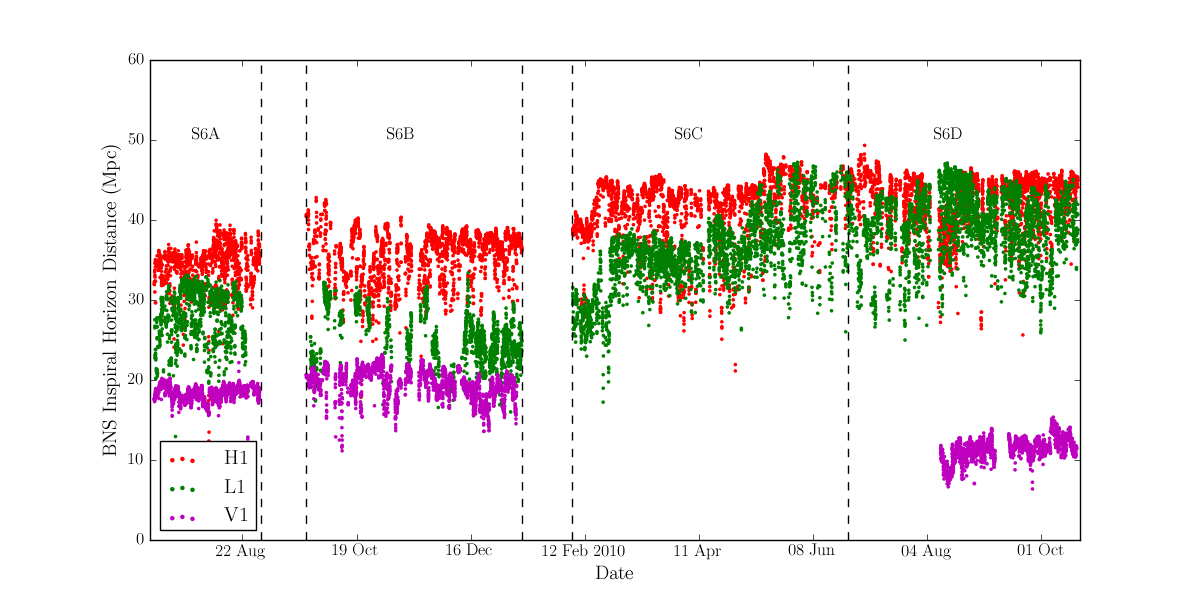
\includegraphics[width=9in]{figures/s6-hzrange_v_time.png}
\end{center}
\caption{The inspiral range for a $1.4/1.4\,\Msun$ \ac{BNS} system at \ac{SNR} $8$ in each \ac{IFO} across \ac{S6}. The range is computed by \texttt{lalapps\_tmpltbank} using equation \ref{eqn:DtoRho}. Each dot represents the range in a $2048\,$s--long analysis chunk.}
\end{figure}
\end{landscape}

\clearpage

\begin{figure}[p]
\begin{center}
\label{fig:s6a_insprange}
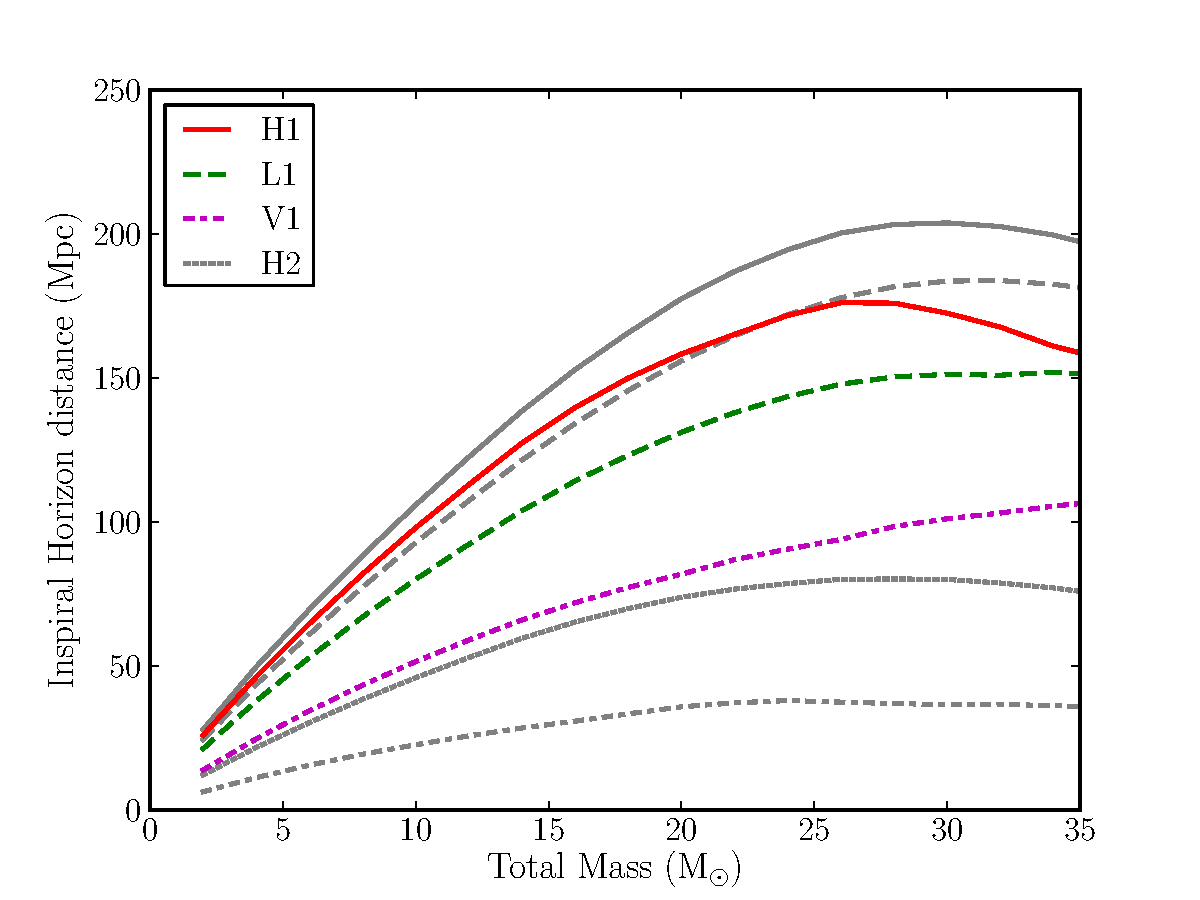
\includegraphics[width=6in]{figures/s6a_insprange.pdf}
\end{center}
\caption{Average inspiral range of S6A. Ranges were computed by \texttt{lalapps\_tmpltbank} using equation \ref{eqn:DtoRho} with $\rho=8$, then averaged over all analysis chunks in the epoch. S6 ranges are in color; best S5 ranges are in gray. Although H2 was not used in \ac{S6}, it is shown for comparison to V1.}
\end{figure}

\begin{figure}[p]
\begin{center}
\label{fig:s6b_pre-hepi_insprange}
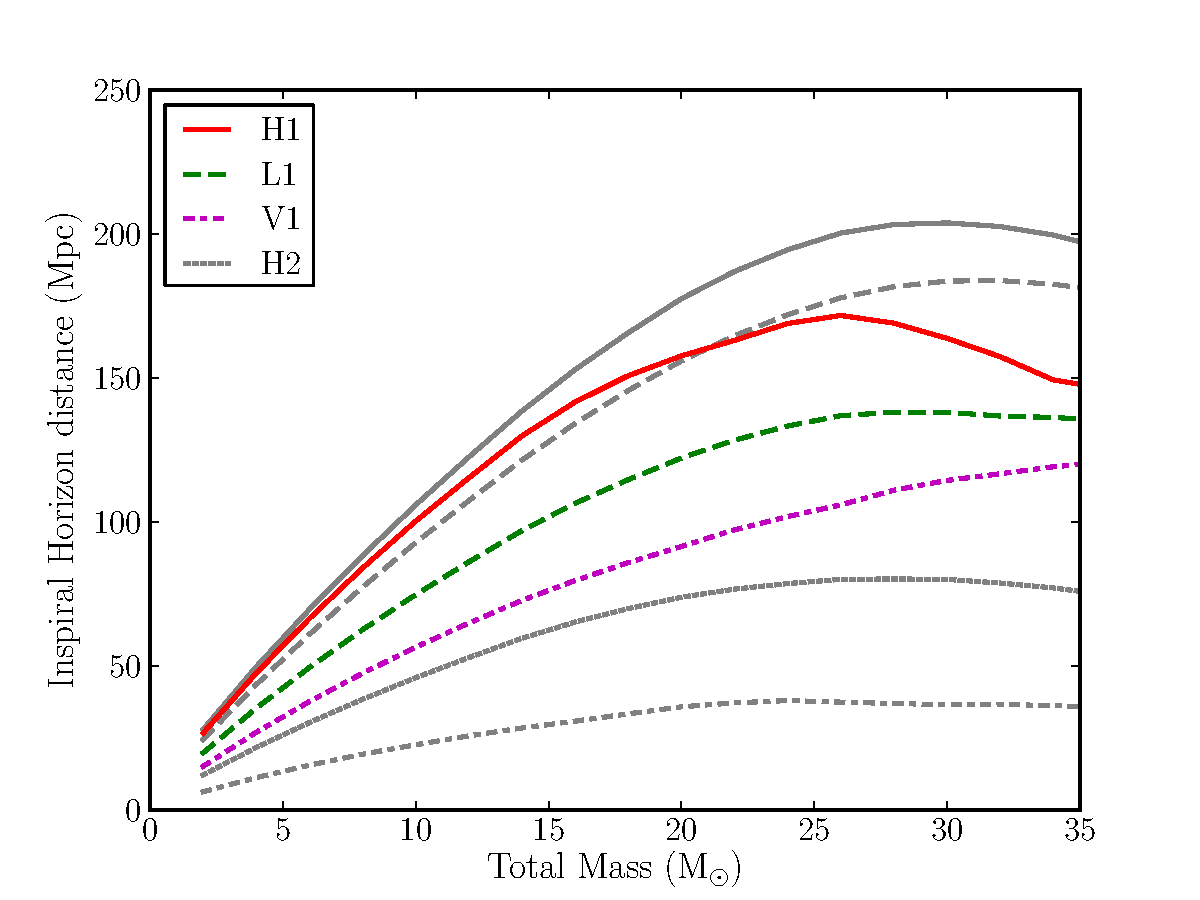
\includegraphics[width=6in]{figures/s6b_pre-hepi_insprange.pdf}
\end{center}
\caption{Average inspiral range of S6B prior to the implementation of \ac{HEPI}. Ranges were computed using the same method as in Figure \ref{fig:s6a_insprange}.}
\end{figure}

\begin{figure}[p]
\begin{center}
\label{fig:s6b_post-hepi_insprange}
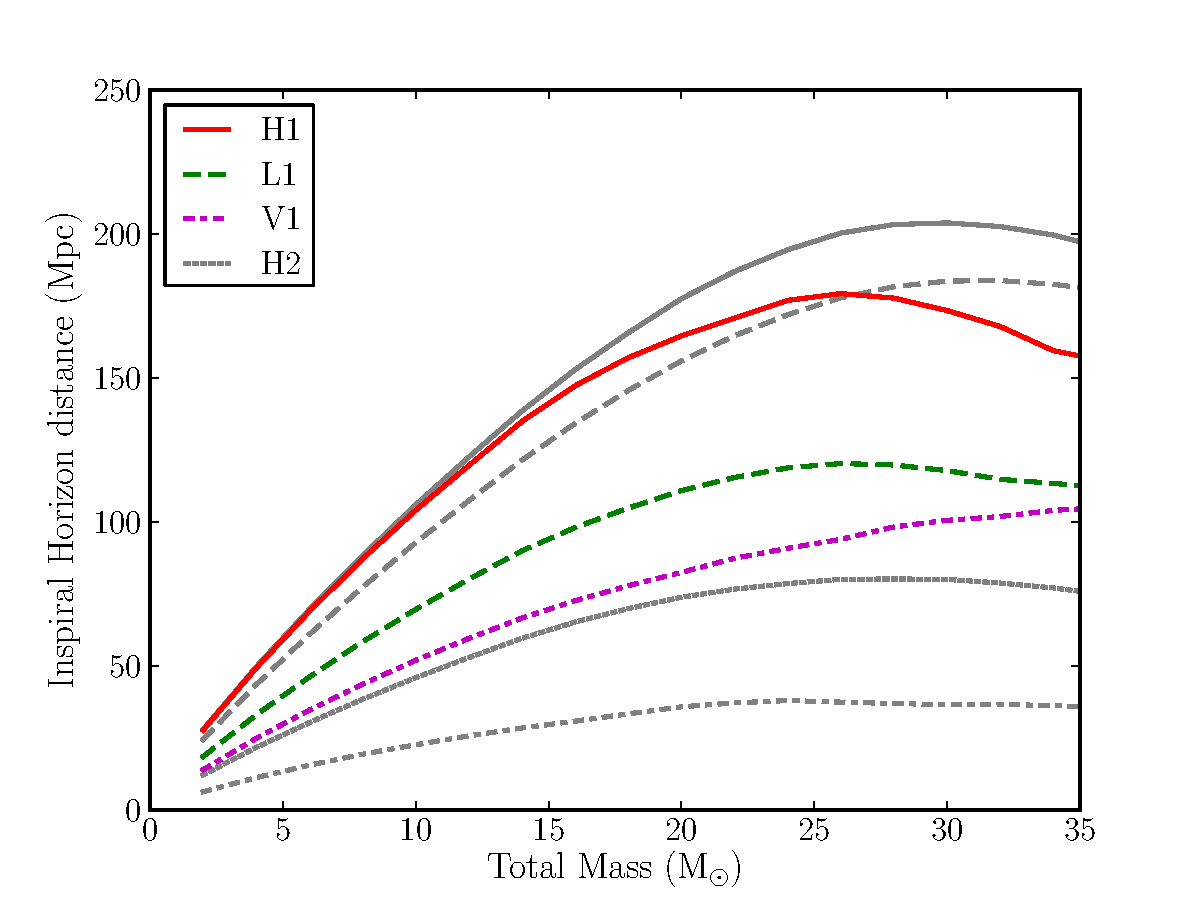
\includegraphics[width=6in]{figures/s6b_post-hepi_insprange.pdf}
\end{center}
\caption{Average inspiral range of S6B after the implementation of \ac{HEPI}. Ranges were computed using the same method as in Figure \ref{fig:s6a_insprange}.}
\end{figure}

\begin{figure}[p]
\begin{center}
\label{fig:s6c_insprange}
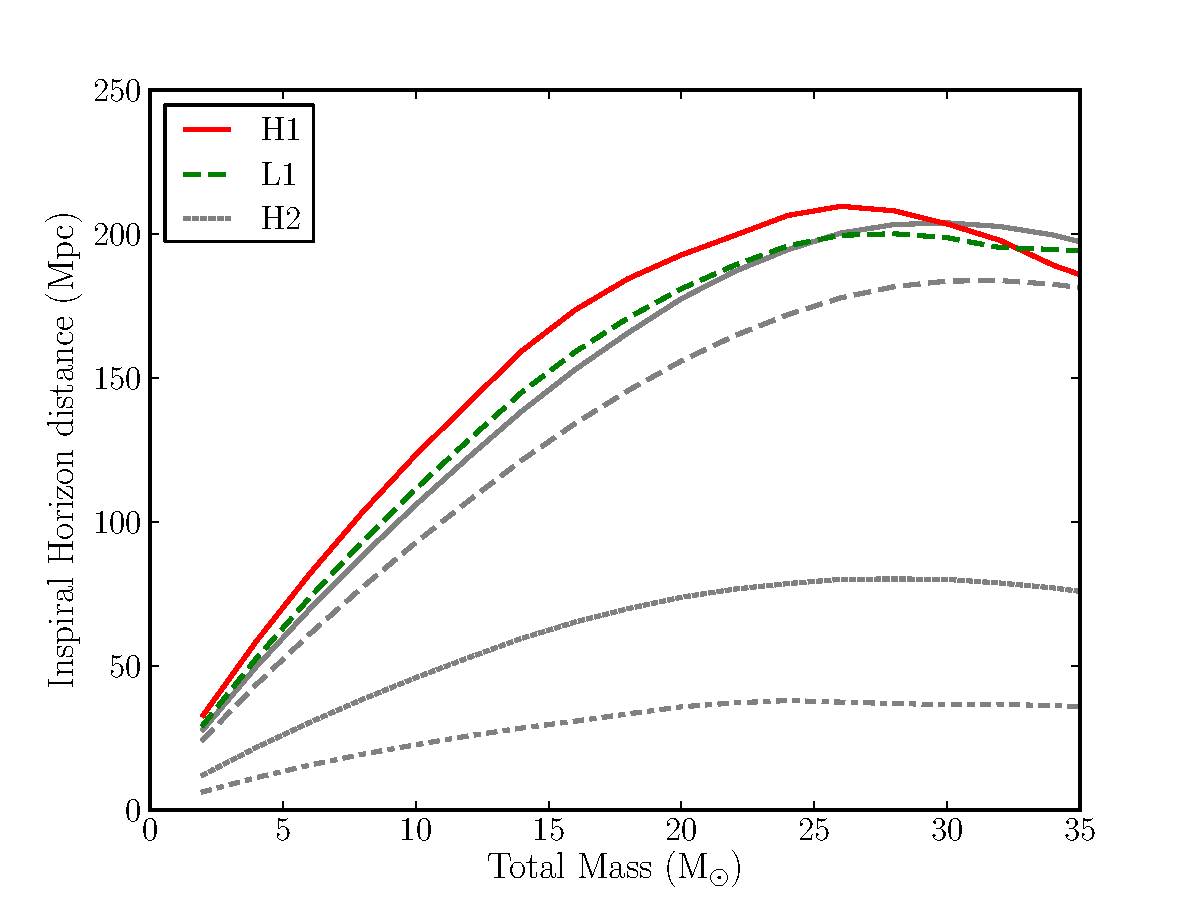
\includegraphics[width=6in]{figures/s6c_insprange.pdf}
\end{center}
\caption{Average inspiral range of S6C. V1 is not shown as it was down for commissioning during this period. Ranges were computed using the same method as in Figure \ref{fig:s6a_insprange}.}
\end{figure}

\begin{figure}[p]
\begin{center}
\label{fig:s6d_insprange}
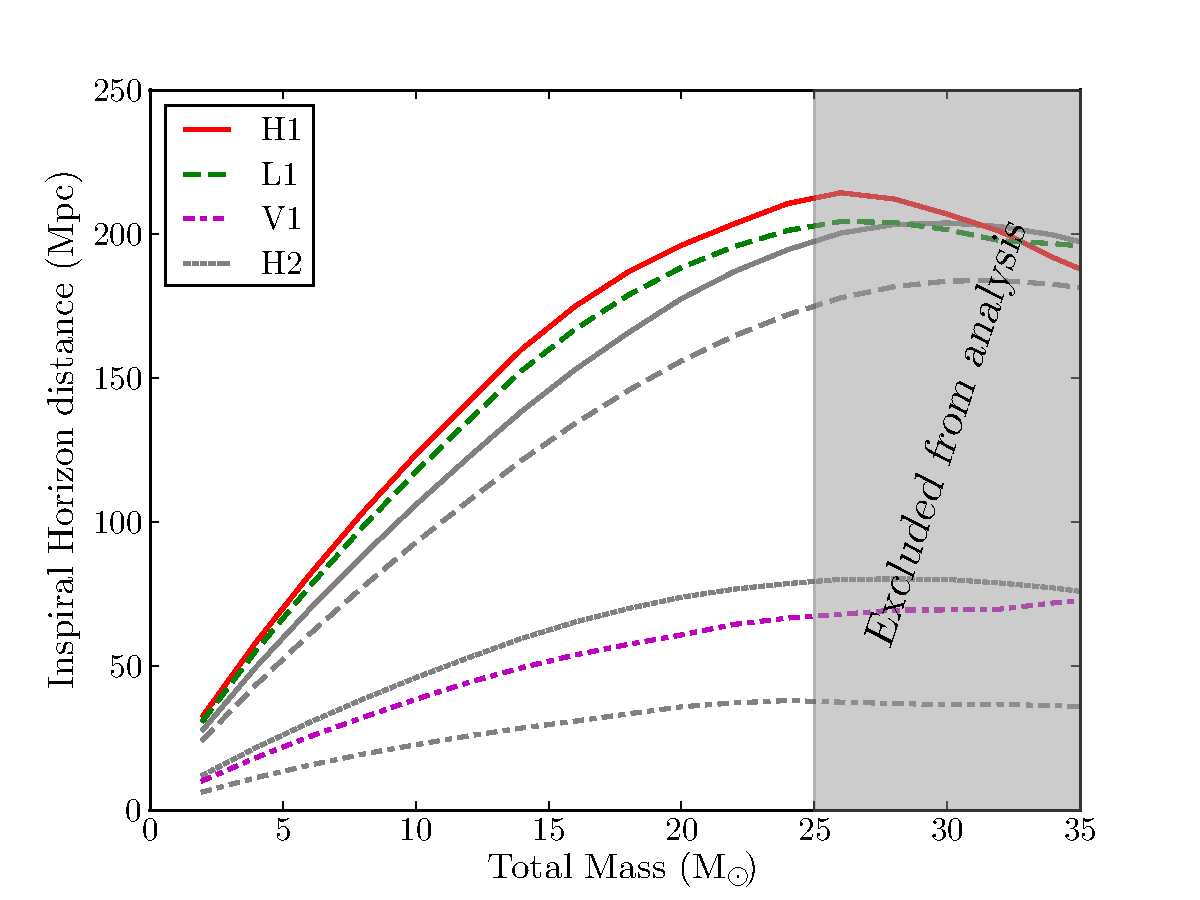
\includegraphics[width=6in]{figures/s6d_insprange_alt.pdf}
\end{center}
\caption{Average inspiral range of S6D. Shaded region indicates the mass range that was excluded in the low mass search for this period. Ranges were computed using the same method as in Figure \ref{fig:s6a_insprange}.}
\end{figure}

\begin{figure}[p]
\center
\subfigure[H1]{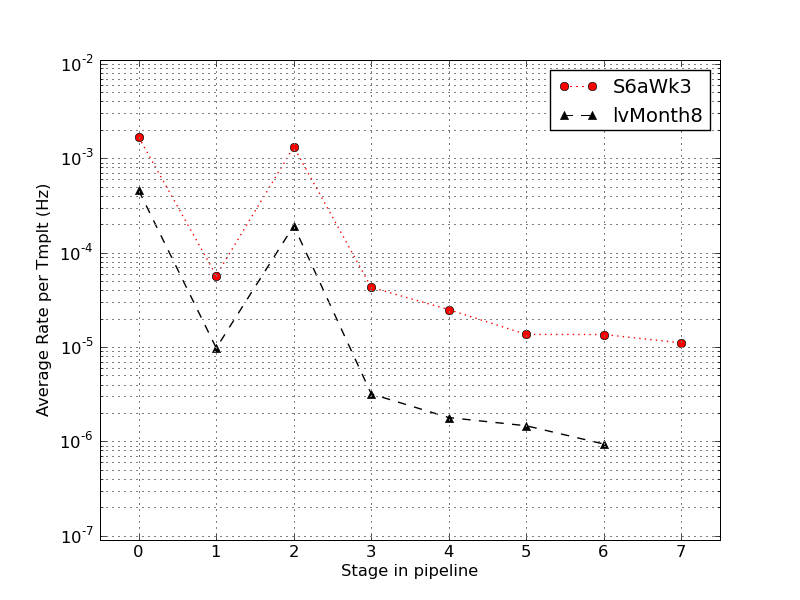
\includegraphics[width=3in]{figures/s6_clusterwin_investigation/H1_average_rate_per_tmplt_comparisons.png}}
\subfigure[L1]{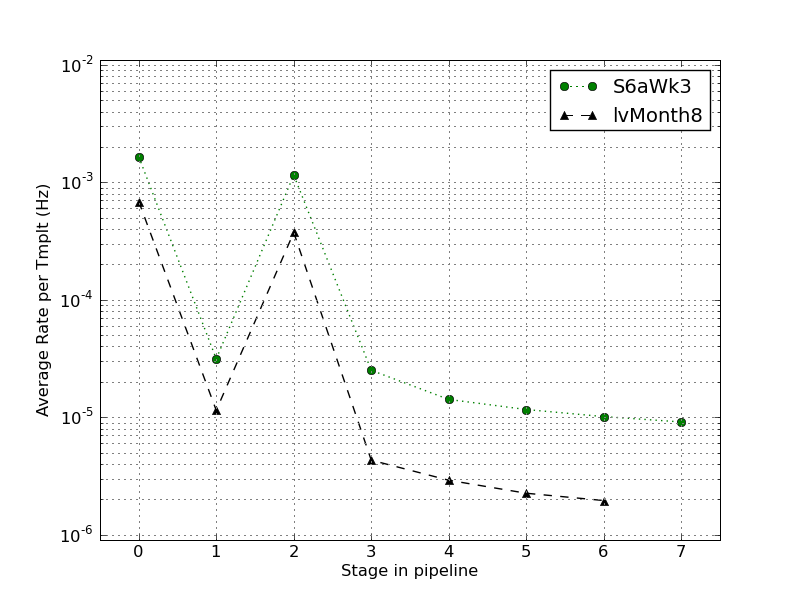
\includegraphics[width=3in]{figures/s6_clusterwin_investigation/L1_average_rate_per_tmplt_comparisons.png}}
\subfigure[V1]{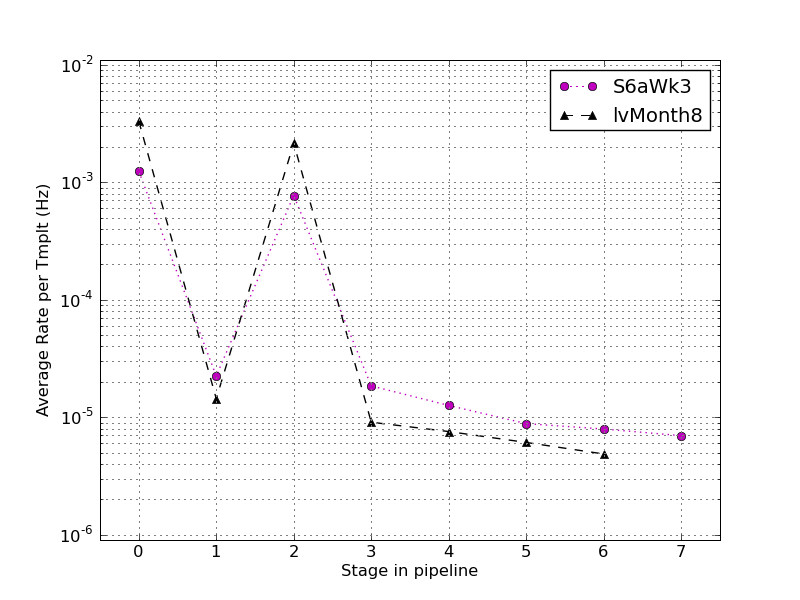
\includegraphics[width=3in]{figures/s6_clusterwin_investigation/V1_average_rate_per_tmplt_comparisons.png}}
\label{fig:avg_rate_per_tmplt}
\caption{The average trigger rate per template in week 3 of S6A as compared to one month from the \ac{S5} LV analysis. Each point represents a different stage in the pipeline: $0 \rightarrow$ \texttt{INSPIRAL\_FIRST}, $1 \rightarrow$ \texttt{THINCA\_FIRST}, $2 \rightarrow$ \texttt{INSPIRAL\_SECOND}, and $3 \rightarrow$ \texttt{THINCA\_SECOND}. Stages $4$--$7$ represent the higher-category vetoes being applied at \texttt{THINCA\_SECOND}; there is an extra stage in S6A because hardware injections were removed by an extra veto-category (between steps $5$ and $6$), whereas in the LV search hardware injections were removed as apart of the CAT2 vetoes (at step $4$).}
\end{figure}

\begin{figure}[p]
\label{fig:roc_cluster_windows}
\center
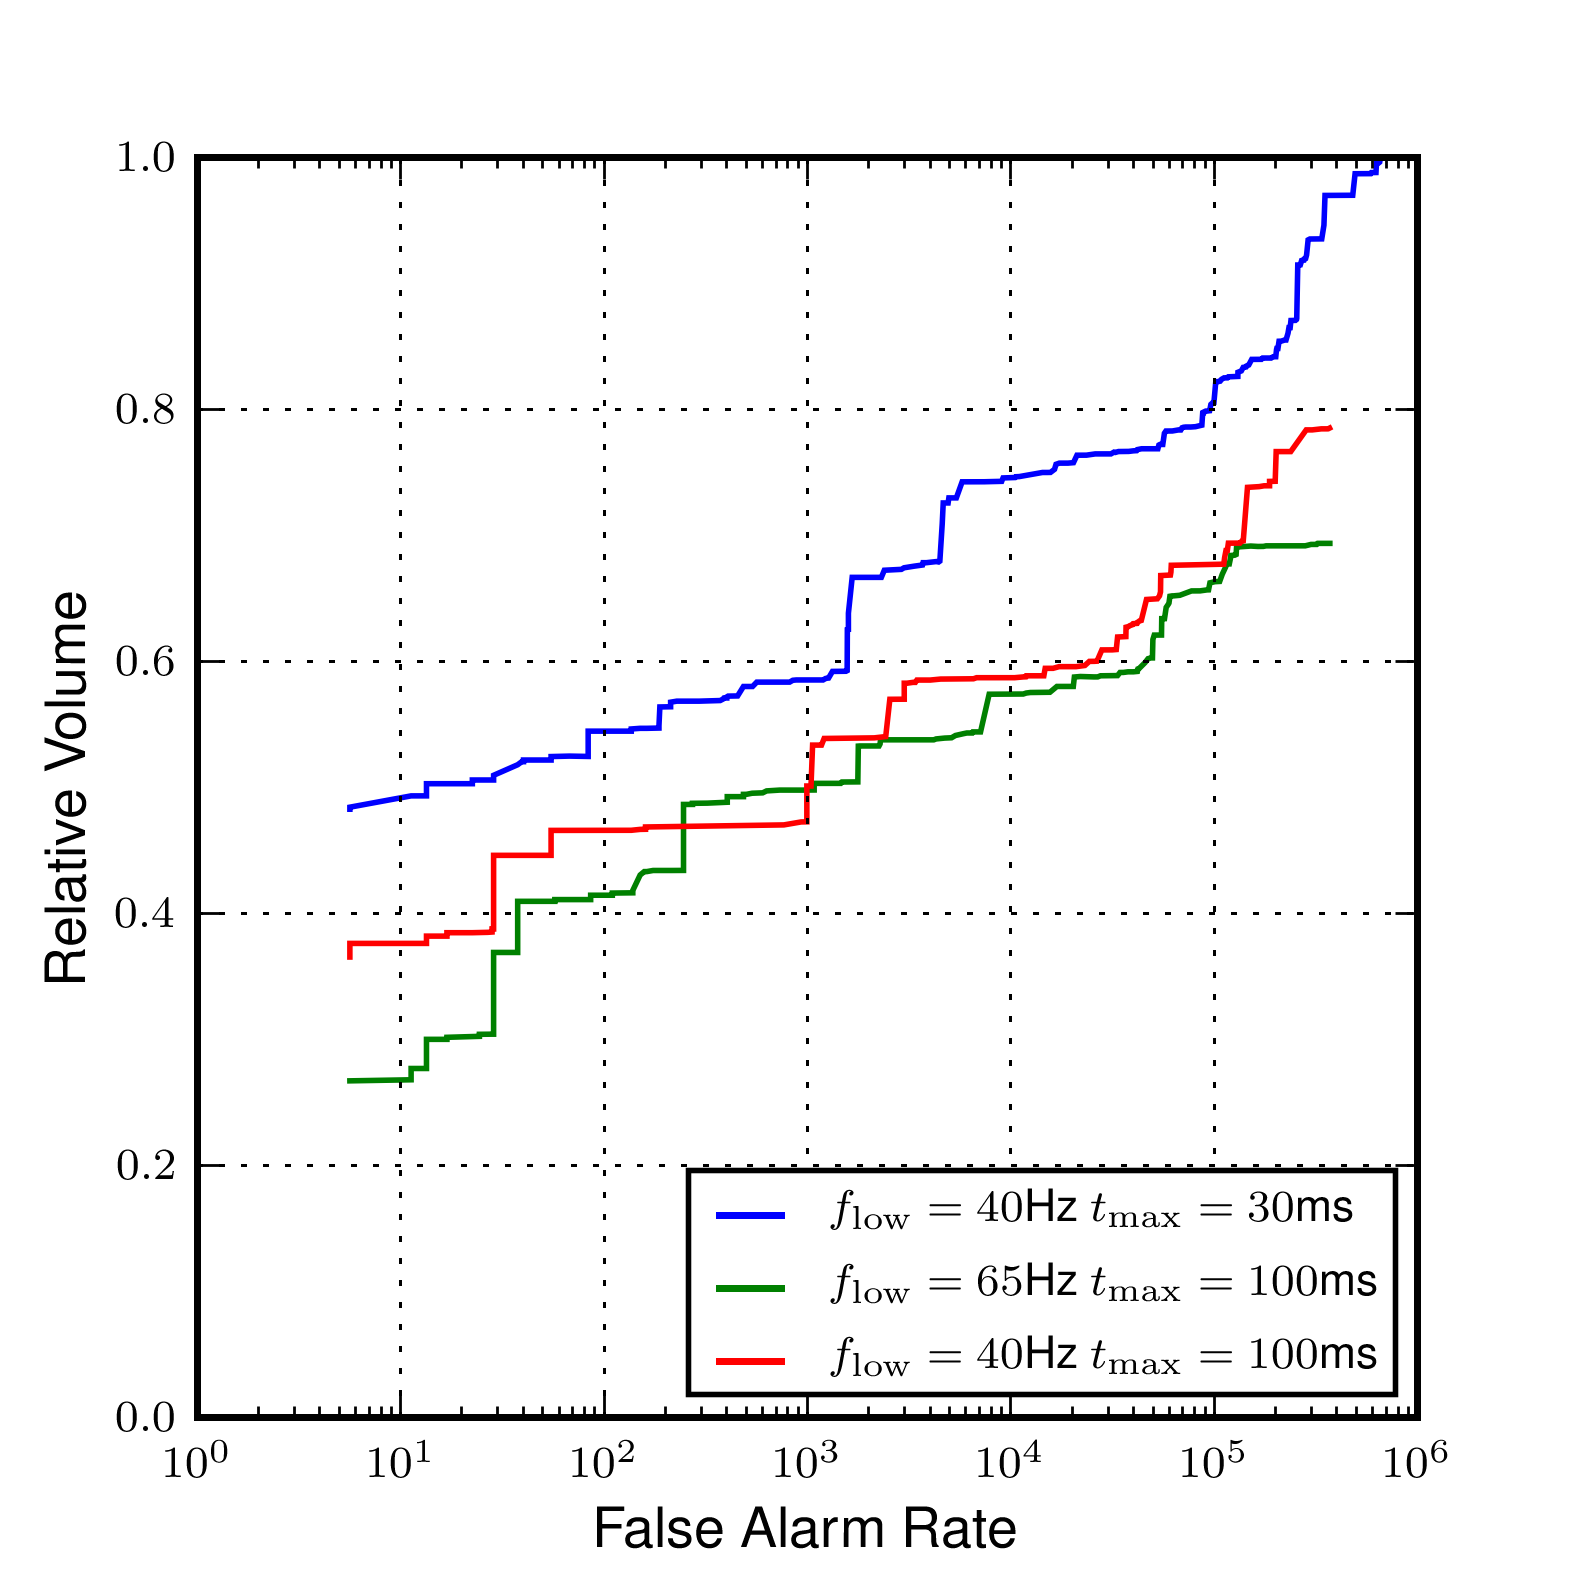
\includegraphics[width=6in]{figures/s6_clusterwin_investigation/s6week3cat4_ROC.png}
\caption{ROC plot from week 3 of S6A using various clustering windows and low-frequency cutoffs.}
\end{figure}

\section{DQ issues}

Review major DQ issues found through S6C and D studies.

\subsection{The ``Spike" Glitch}
Loud, short, transients in L1 OMC. Show one of Andy's time-series plots. Also show an Omega scan, and \ac{CBC} triggers created by it. Unable to determine cause. We resolved to create an \ac{SNR} > 250 flag, and veto at CAT3. Duncan MacCleod and I were supposed to study the effect on nearby injections, but it appears to have never finished.

\subsection{Decreasing the Upper End of the Template Bank}
High mass and low mass seraches overlapped in the region $25 \leq \mtotal/\Msun \leq 35$. Tom found that the high mass search did a better job recovering injections in this range. I did a study to see how much better the low-mass search would do with a smaller bank. Found that it was better, but not by enough to warrant re-doing runs up to that point. Show plotfm plots that I created. ROC curves?

During this investigation I find that nearby missed injection that appeared to be in clean time. Nothing became of it though; should I discuss this?

\subsection{V1 Doubles in S6D Triple Time}

V1 was glitchy and had poor range when came back up for VSR3. Summarize my study of what we gained/lost by throwing out H1V1 and L1V1 triggers in triple time. ROC plots? 

\section{Results}

Give loudest events. From re-runs? Copy from S6 paper?

\subsection{The Blind Injection}

Copy from S6 paper? Talk about extrapolation. Add detail about how extra slides were done. Remove discussion of parameter estimation.

\subsection{Conclusions}

In the S6 paper I draw on the upper-limits in the conclusion. Can I show preliminary upper limits?

\section{Extra Stuff}

(Next chapter)

The other investigation was the LIGO South investigation of whether or not we can detect at SNR 8 with two detectors. The wiki for this is linked from the April 13, 2010 CBC minutes. It was done using S5 data, so it doesn't seem to belong in this chapter. S5 chapter? Or at all? I allude to it in Chapter 2 we showing plots of snr and newsnr.

